\documentclass[a4paper,twoside]{article}

\usepackage{RR}
\usepackage{hyperref}
%\usepackage[frenchb]{babel}
%\usepackage[T1]{fontenc} % avec T1 comme option  d'encodage c'est ben mieux, surtout pour taper du français.
\usepackage[utf8]{inputenc}
\usepackage[table]{xcolor}
\usepackage{color}
\usepackage{graphicx}
\usepackage{amsmath, amsthm}
\usepackage{stmaryrd}
\usepackage{lscape}

\usepackage{url} \urlstyle{sf}%
\usepackage{graphicx}%
\usepackage{subfigure}
\usepackage{listings}%

\lstset{%
  basicstyle=\scriptsize,%
  numbers=left,
  %columns=fullflexible,%
  language=XML,%
  %frame=shadowbox,
    frame=lbtr,%
  frameround=tttt,%
  tabsize=2,
  breaklines=true
}%
\usepackage{tikz}
\usetikzlibrary{decorations.pathreplacing,positioning}
\usepackage{array}
\usepackage{xspace}

\newcommand{\ie}[0]{{\em i.e.},\xspace}
\newcommand{\vs}[0]{{\em vs.}\xspace}
\newcommand{\eg}[0]{{\em e.g.},\xspace}
\newcommand{\etal}[0]{{\em et al.}\xspace}
\newcommand{\wrt}[0]{{\em w.r.t.}\xspace}
\newcommand{\aka}[0]{{\em a.k.a.}\xspace}

\sloppy

%%% FORMAT DOCUMENT

\def\textfraction{0}
\def\floatpagefraction{1}
\def\topnumber{3}
\def\bottomnumber{3}
\def\totalnumber{3}
\def\topfraction{1}
\def\bottomfraction{1}

%%.
\usepackage{bold-extra,graphicx,latexsym,mathrsfs,subfigure,xspace}

\usepackage{color}
\usepackage{array}
\usepackage{longtable}
\usepackage{calc}
\usepackage{multirow}
\usepackage{hhline}
\usepackage{ifthen}

\usepackage{hyperref}

\newcolumntype{M}[1]{>{\raggedleft}m{#1}}
\newcommand{\discovery}{DISCOVERY\xspace}

%% CT %%
\newcommand{\ftodo}[2][\relax]  % \TODO[editor]{text} 
  {\ensuremath{{}^{\mbox{\tiny\bf #1}}}~\textbf{#2}}

\begin{document}

\RRNo{480}
\RRdate{February 2016}

\RRprojet{DISCOVERY IPL}

% \author{Adrien L?bre\inst{1,3} \and Jonathan Pastor\inst{1,3} \and Marin Bertier \inst{2,3} \and Fr?d?ric Desprez\inst{3} \and Jonathan Rouzaud-Cornabas\inst{3} \and C?dric Tedeschi \inst{3,4}\and Paolo Anedda\inst{5} \and Gianluigi Zanetti\inst{5} 
% \and Ramon Nou\inst{6} \and Toni Cortes\inst{6} \and Etienne Riviere\inst{7} \and Thomas Ropars\inst{8}}
% \institute{LINA / Mines Nantes, France 
% \and IRISA / INSA de Rennes, France
% \and INRIA, France
% \and IRISA / Universit? de Rennes 1, France
% \and Center for Advanced Studies, Research and Development in Sardinia (CRS4), Italy
% \and Barcelona Supercomputing Center (BSC), Spain
% \and Universit? de Neuch?tel (UniNe), Switzerland
% \and Ecole Polytechnique F?d?rale de Lausanne (EPFL), Switzerland} 

%
% Title and Authors
%
\RRauthor{
A. Lebre\thanks[Inria]{Inria, France, Email: \url{FirstName.LastName@inria.fr}}\thanks[EMN]{Mines Nantes/LINA (UMR 6241), France.}%\inst{1} 
\and 
J. Pastor\thanksref{Inria}\thanksref{EMN} 
\and 
Frederic Desprez\thanksref{Inria}  
}

\authorhead{A. Lebre et al.}

\RRtitle{Révisiter les mécanismes internes du système OpenStack en vue d'opérer des infrastructures de type nuage massivement distribuées}
\RRetitle{
A Ring to Rule Them All - Revising OpenStack Internals to Operate Massively Distributed Clouds}%\thanks{This report ....}}
\titlehead{The DISCOVERY Initiative}

%\RRnote {XXXX}

\RRkeyword{Fog, Edge Computing, 
Peer To Peer,
Self-*,
Sustainability,
Efficiency,
OpenStack, 
Future Internet.
}

\RRmotcle{Calcul utilitaire basé sur la localité, systèmes pair-à-pair, self-*, durabilité,OpenStack 
Internet du futur}

%
% Abstract
%
\RRabstract{

  {\small 

The deployment of micro/nano data-centers in network point of presence offers an opportunity to deliver a more sustainable and efficient infrastructure for Cloud Computing. Among the different challenges we need to address to favor the adoption of such a model, the development of a system in charge of turning such a complex and diverse network of resources into a collection of abstracted computing facilities that are convenient to administrate and use is critical.

In this report, we introduce the premises of such a system. The novelty of our work is that instead of developing a system from scratch, we revised the OpenStack solution in order to operate such an infrastructure in a distributed manner leveraging P2P mechanisms. More precisely, we describe how we revised the Nova service by leveraging a distributed key/value store instead of the centralized SQL backend. We present experiments that validated the correct behavior of our prototype, while having promising performance using several clusters composed of servers of the Grid'5000 testbed. We believe that such a strategy is promising and paves the way to a first large-scale and WAN-wide IaaS manager.

}
}

\RRresume{

  {\small 

La tendance actuelle pour supporter la demande croissante d'informatique
utilitaire consiste à construire des centres de données de plus en plus grands,
dans un nombre limité de lieux stratégiques. Cette approche permet sans aucun
doute de satisfaire la demande actuelle tout en conservant une approche
centralisée de la gestion de ces ressources, mais elle reste loin de pouvoir
fournir des infrastructures répondant aux contraintes actuelles et futures en
termes d’efficacité, de juridiction ou encore de durabilité.  L’objectif de
l'initiative DISCOVERY\footnote{\url{http://beyondtheclouds.github.io}} est de
concevoir le \emph{LUC OS},  un système de gestion distribuée des ressources qui permettra de
tirer parti de n’importe quel n\oe ud réseau constituant la dorsale d’Internet
afin de fournir une nouvelle génération d’informatique utilitaire, plus apte à
prendre en compte la dispersion géographique des utilisateurs et leur demande
toujours croissante. 

Après avoir rappelé les objectifs de l'initiative DISCOVERY et expliqué
pourquoi les approches type fédération ne sont pas adaptées pour opérer une
infrastructure d'informatique utilitaire intégrée au réseau, nous présentons les
prémisses de notre système.  Nous expliquerons notamment pourquoi et comment
nous avons choisi de démarrer des travaux visant à revisiter la conception de
la solution Openstack. De notre point de vue, choisir d'appuyer nos travaux sur
cette solution est une stratégie judicieuse à la vue de la complexité des
systèmes de gestion des plateformes IaaS et de la vélocité des solutions
open-source. 
}
}

\URRennes
\makeRR

%%%

\section{Introduction}

\subsection{Massively distributed cloud}

\begin{itemize}

	\item A massively distributed cloud targets management of thousand of hosts around a wide territory.	
	
	\item This scale order is currently reached by file sharing systems like bittorrent.

	\item At this scale, failure becomes the norm.

	\item Recent works propose to leverage on peer to peer overlay.

	\item Some peer to peer overlays can take advantage of locality. It enables to build systems that can take
		  into account network bandwidth and latency.

	\item We propose to leverage on locality based peer to peer mechanisms to reach an high scalability IaaS.

\end{itemize}

\subsection{Toolkit for IaaS}

\begin{itemize}

	\item A toolkit is a building block that can be used for the construction of systems.

	\item The objective of a toolkit is to provide "state of the art" solutions to known problems. It enables the
		  focus on "Top level" works.

	\item It provides a set of components, which once assembled constitute an operational system.

	\item Recent studies of "state of art IaaS systems" (Openstack, Cloudstack, OpenNebula, ...) showed that they
		  were constructed over same concepts. It enables the design of IaaS toolkit.

	\item The massively distributed IaaS toolkit will provides "state of the arts" mechanism to solve both scalability and locality points.

	\item The toolkit will have to integrate well on existing systems: we propose to leverage Openstack project.

\end{itemize}


\section{Revising OpenStack}
\label{sec:leveraging-openstack}

OpenStack is an open-source project that aims at developing a complete cloud management
system. Similary to the reference architecture described in the previous Section, it is
composed of several services, each one dealing with a particular
aspect of a Cloud infrastructure as depicted in Figure~\ref{fig:openstack}.

\begin{figure}[htbp]
        \centering
        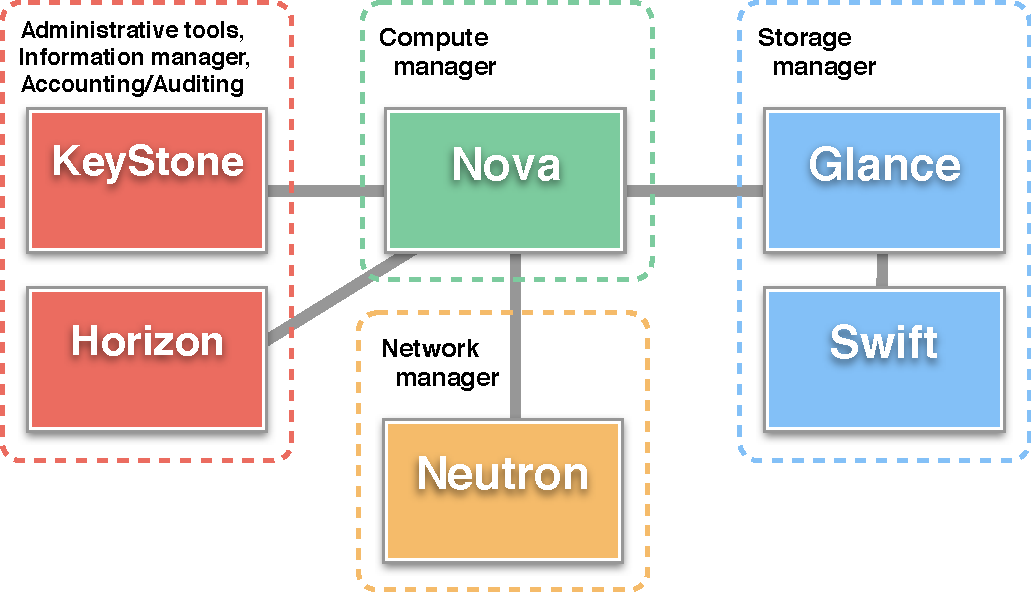
\includegraphics[width=6cm]{figures/OpenStack_architecture.pdf}
\vspace*{-.3cm}
        \caption{Services composing OpenStack.}
        \label{fig:openstack}
\vspace*{-.3cm}
\end{figure}


OpenStack relies on two kinds
of nodes: controller and compute node. The former is in charge of managing and
distributing work to the latter that provides computing/storage resources to end-users. In
other words, the controllers correspond to the different services introduced in the
previous section while the compute nodes host the VMs.

From the software point of view, the OpenStack architecture is based on the ``shared
nothing" principles: each controller (\ie each service) is connected to the others via two
different way:

\begin{itemize}
   \setlength{\itemsep}{0pt}
  \setlength{\parskip}{0pt}
   \setlength{\parsep}{0pt}
\item \textbf{A messaging queue} that enables the collaboration between sub-services of a
  controller.
\item \textbf{A SQL database} (DB) that stores inner states of a controller.
\end{itemize}

Finally, the controllers interact with each other through REST APIs or directly by accessing
the inner-state that are stored in the differents DBs.
%\AL[JP]{Is it correct ? How the controllers interaact/collabore ?}

Considering the current structure of OpenStack, the main limitation to make it distributed
is related to the SQL databases. Indeed, while OpenStack relies on the
RabbitMQ messaging service, which is articulated around a centralized
broker, there are few implementations of  P2P messaging
service such as ActiveMQ~\cite{activemq:2011} or ZeroMQ~\cite{zeromq:2013} that would be adapted to the LUC requirements.
% \section{Towards a fully distributed OpenStack deployment}
%
% The discovery initiative targets the delivery of an utility computing platform
% that will be working on top of existing network backbone facilities. Starting
% the development of such a platform from zero would require a titanic effort: in
% order to spare a giant development time, the Discovery initiative proposes to
% leverage the OpenStack project: this will serve as the foundation of the
% LUC-OS.
%
% In order to structure the LUC-OS on a fully distributed peer to peer
% functionning, OpenStack would be required to be fault tolerant and to be able to
% fit on a multi-site configuration. In the current situation, it requires some
% adaptations: in this section we propose some modifications that
% have been introduced in the Nova controller, to meet the two
% aforementioned criterions.
%
% \subsection{Replacing the relational backend by a Key/value store}
%
% From today's perspective, most of the OpenStack deployment are involving few
% nodes, thus not requiring more thant one controller. However, to meet the fault
% tolerance criterion, one needs to use \textit{High availibility} deployment by
% combining two components \textit{HAProxy} (load balancing) with
% \textit{Galera} (Relational database replication).
The first way to bypass the MySQL limitation is to
% a controller between distinct locations,
%\ie to be able to scale in/out the services it offers, is to
deploy each controller DB on each location and to synchronize the different DB
instances with a dedicated mechanism~\cite{kemme:vldb2010}. By such a mean, when a
controller processes a request and performs some actions on one site, changes in the
inner-state are also propagated to all the other locations. From a certain point of view,
it gives the illusion that there is only one DB for each service. Although the technique
described has been used in different proof-of-concepts, current DB synchronization
mechanisms are not scalable enough to cope with a LUC infrastructure deployed on large
number of geographical sites.

Another approach is to replace the DBs used in OpenStack by a more suitable storage
backend that would provide a better scalability. Distributed Hash Tables (DHTs) and more
recently key/value systems built on top of the DHT concept such as
\emph{Dynamo}~\cite{decandia:dynamo} have demonstrated their efficiency in terms of
scalability and fault tolerance properties.
%
In light of this, we have revisited the Nova controller, \ie the VM manager of OpenStack,
in order to to replace the current MySQL DB system by \textit{REDIS} ~\cite{han:2011},
a \textit{key/value store}.
% that extends the principles followed by the \textit{Dynamo}. %with more advanced storage and query features.
Technically speaking, we modified the Nova database driver. Indeed, the  Nova software architecture has been
organised in a way which ensures that each of its sub-services does not directly manipulate the database: they have an indirect
access through a service called ``nova-conductor" which in turn works with an
implementation of the \textbf{"nova.db.api"} programming interface. Developers of Nova
provide an implementation of this interface that is using \textit{SQLAlchemy} to
manipulate a relational database. We developed a second implementation of this interface
that replaces every call to the \textit{SQLAlchemy} by a call to a
custom key/value store
driver.  This enables  Nova's services to work with REDIS by only changing the
database driver, limiting the level of intrusiveness in the original source code.
Thanks to this modification, it is possible to instanciate  a distributed
cloud and operate it through a single instance of OpenStack composed
of several Nova controllers deployed on distinct sites.
Figure~\ref{fig:newnova} depictes such a deployment.
%
Each controller executes a REDIS instance that is configured to work in
a clustering way with other instances.
One or several controllers can be deployed on each site according to
the expected demand in terms of end-users. Finally, a controller can be
deployed either on a dedicated node or be mutalized with a compute
one as illustrated for Site 3. We higlight that any controller can
provision VMs by orchestrating services on the whole infrastructure and not only on the site
where it is deployed. Such a behavior is possible thanks to the AMQP
bus and the key/value store that go through all controllers.
%
Finally, it is noteworthy that key/value stores that
focus on high-availability and partition tolerance criteria like
Cassandra~\cite{lakshman:2010} would be more appropriate than REDIS
for a production deployment. We chose REDIS for its usage simplicity.

\begin{figure}[htbp]
        \centering
\vspace*{-.4cm}        \hspace*{-.2cm}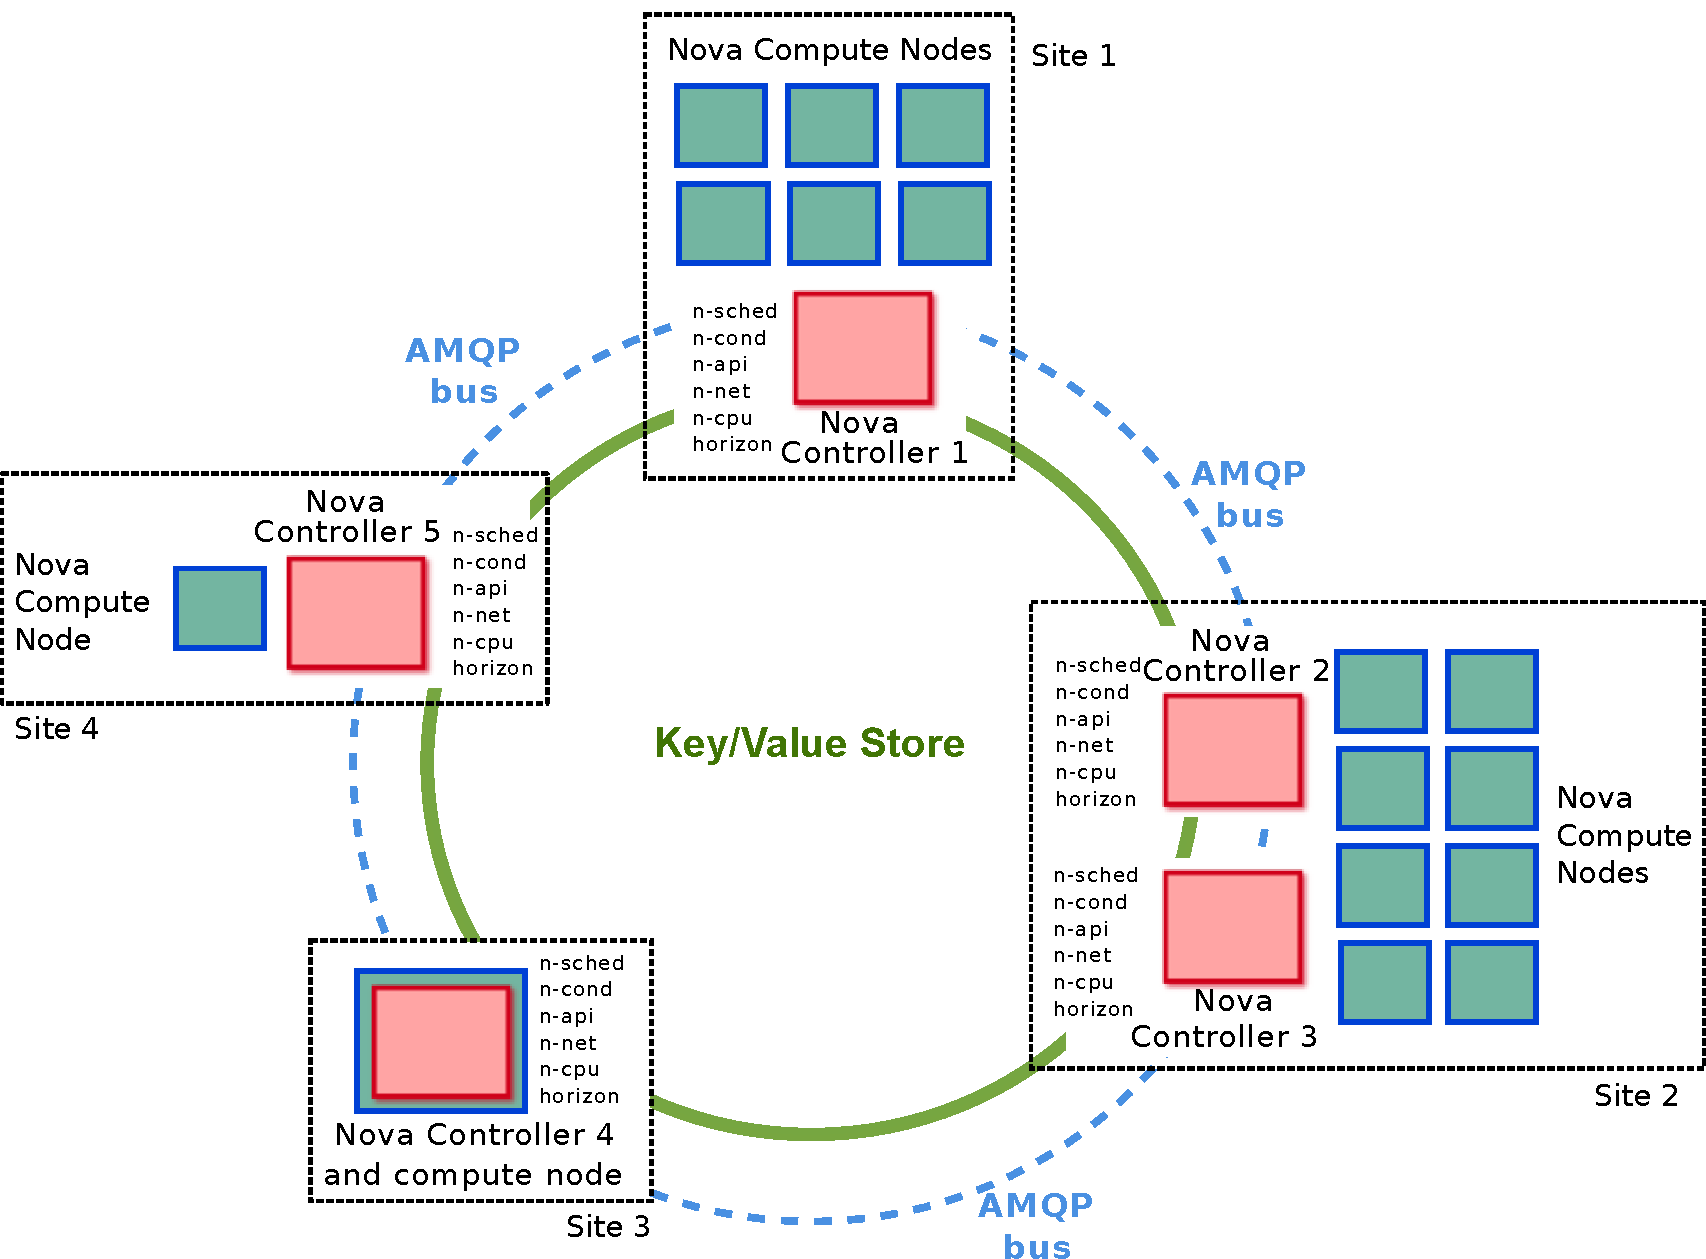
\includegraphics[width=.51\textwidth]{figures/OpenStack_distributed.pdf}
        \caption{Nova controllers are connected through a shared key/value backend
        and the AMQP bus.}
      \label{fig:newnova}
\vspace*{-.3cm}
\end{figure}

Our prototype is under evaluation.
However, preliminary experiments  have been performed throughout 4
sites of Grid'5000  including 12 compute nodes  and 4 controllers
overall. While this
infrastructure was rather small in comparison to our target, it aimed
at validating the interconnection of several controllers WANwide and
the correct behaviour of  OpenStack using our noSQL backend.
Our prototype suceeded to provision 500 VMs in 300 seconds
(each controller creating 125 VMs in parallel).
A second experiment validated the provisionning
of 2000 VMs in less than 30 min.  We are currently performing comparisons
between OpenStack using the historical MYSQL backend \textit{v.s.,}
using a key/value store backend. Our goal is to validate that
manipulating internal states of Openstack through
a noSQL deliver performances in the same order of the MySQL
ones.


\section{Experimental validation on Grid'5000}
\label{sec:eval}

The validation of our prototype has been performed thanks to the Grid'5000
testbed \cite{grid5000}. Grid'5000 is a large-scale and versatile experimental
testbed for experiment driven research in Computer Science, which enables
researchers to get an access to a large amount of computing resources
($\sim$ 1000 nodes spread over 10 sites). This delivery of computing resources
takes the form of bare-metal machines, on which fully customised software stacks
can deployed, thus giving a very fine control of the experimental conditions.

Various tools have been developed to provide an ease of use, such as monitoring
information about networking and power consumption or programming libraries to
fine tune each aspect composing an experiment. With this in mind, we developed
our prototype using the Execo framework \cite{imbert:hal-00861886} which helped
us to deploy and configure each node composing our chosen software stack (Ubuntu
14.04, a modified version of OpenStack "devstack", and the RIAK key/value store).

Our validation scenario has consisted in the creation of 30 VMs
through 10 different Nova controllers deployed on one cluster located
in Nantes. This experiment enabled us to confirm that OpenStack's
services were working correctly with the key/value store.
% that the relational backend
%used by the several components can be satisfactorily replaced by this
%new distributed key/value system.
Although further experiments are
required to test the scalability as well as the effect
of geographical distances on the reliability and efficiency, we are
confident about our approach as several distributed key/value stores
are already used WANWide.

% \AL[JP]{Finalize the text of this section, please be consistent the
%   announcement at the end of the introduction}
% Several test-cases with 10 nodes to evaluate
% the efficiency of the new framework:\begin{inparaenum}[1\upshape)]
% \item 1 site, 1 controller, 9 compute nodes
% \item 1 site, 10 controllesr, 0 compute node
% \item 2 sites, 1 controller/by site, 4 compute nodes/by site
% \item and 2 sites, 5 controllers/by site, 0 compute nodes/by site
% \end{inparaenum}



%test infrastructure is a tedious task if one has to do it
%manually. In order to simplify tests, we create a tool based on \texttt{Execo}
%\cite{imbert:hal-00861886} that: find a time slot when the resources
%are available on the several sites.
% deploy Ubuntu 14.04 on all the nodes, install RIAK DB and setup
% our modified version of devstack (with automatic node configuration), and
% finally start the distributed OpenStack infrastructure. The duration of the
% deployment is around 1 hour, depending on the cluster hardware and the
% total number of nodes. Finally, the tool provides some options that simplifies
% the management of the different test-cases, namely the number of sites,
% controller by site and compute nodes by site.

%\begin{figure}[h!]
%    \centering
%    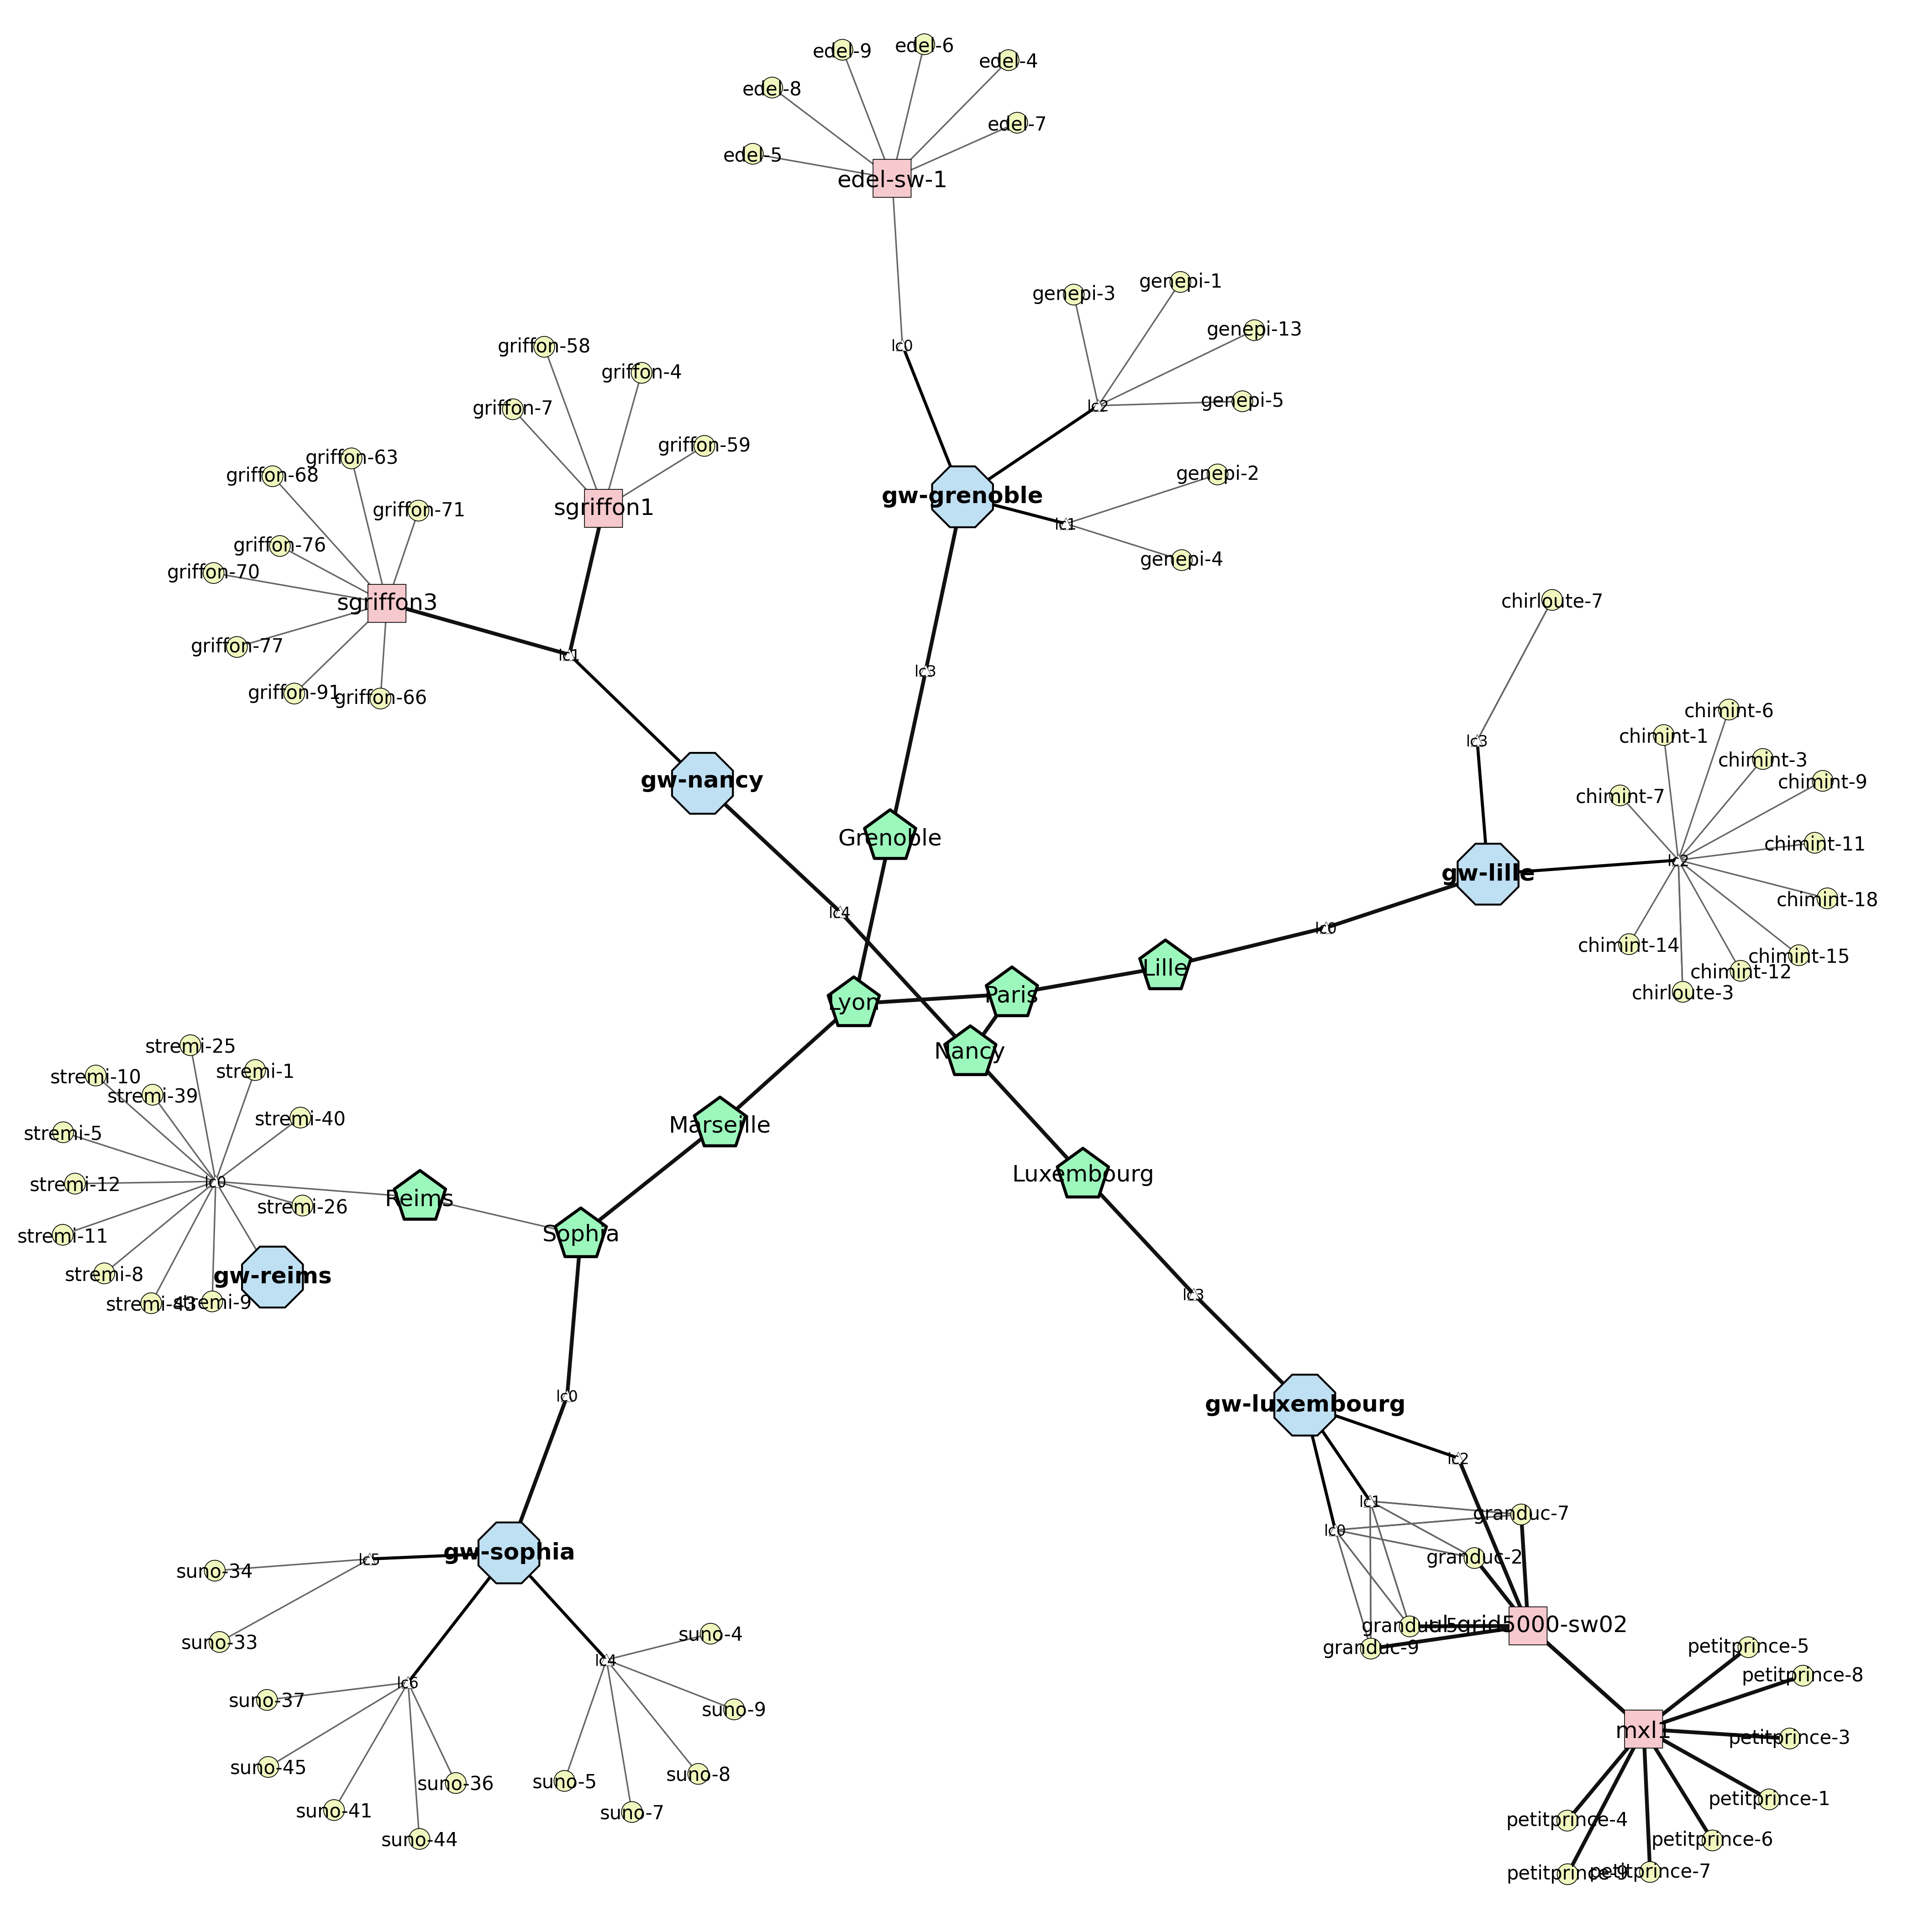
\includegraphics[width=7cm]{figures/6_sites.png}
%    \caption{Test-cases on the Grid'5000 platform involving 6
%    geographically-spreaded sites each hosting 2 controllers and 10 computes
%    nodes.}
%\end{figure}


%\subsubsection{Test-cases}
%\paragraph{Monosite}
%\paragraph{Multisite: 1 controller per site}
%\paragraph{Multisite: 10 controllers per site}


\section{On-going Work}
\label{sec:ongoing_work}

While the Nova revision we presented in the previous
sections is a promising proof-of-concept toward widely distributed OpenStack
infrastructures, there are remaining challenges that need to be tackle.

%First, it is critical to study whether similar changes can be achieved on other components.
%Second, the notion of locality does not exist in our current implementation.
%That is, any request can be served by any controller available, leading to the creation of a VM anywhere in the infrastructure.

In  this section,  we present  two on-going  actions that  aim at  deepening the
relevance of our approach. First,  we show that existing seggregation mechanisms
provided by OpenStack are not satisfactory  when it comes to reducing inter-site
communications.
%  in  order to  improve  networking  efficiency of  a  multi-site OpenStack  deployment.
In  response,  two actions  could be  made:  on one  hand
introducing  networking  locality  in  the   shared  databases  and  the  shared
messaging, on the other hand distributing remaining services of OpenStack.

%While the achievement of such
%changes are under heavy development, we believe that our approach is promising
%enough to favor the adoption of the distributed cloud model supervised by a
%single system.

Second, we discuss the preliminary study we  made on the Glance image service to
investigate whether it is possible to apply similar modifications to the ones we
performed on Nova. Such a validation is  critical as Glance is a key element for
operating a production-ready IaaS infrastructure.

These two actions clearly demonstrate that our approach is promising
enough to favor the adoption of the distributed cloud model supervised by a
single system.

\subsection{Locality Challenges / $\mu$cro DCs Segregation}

%% Even if this article has demonstrated that the relational database used by Nova
%% could be replaced by a non relational key/value store, a more advanced
%% validation of this change is required and the question of which metrics to use
%% remains. On one hand, a larger deployment involving more geographical sites
%% would be more demonstrative, on the other hand the changes we introduced have
%% been have been motivated by more than overall scalabity, but also fault
%% tolerance and reduction of response times when processing API requests.

%% \subsection{Distributing the remaining services of OpenStack}

%% As introduced in section \ref{leveraging-openstack}, the other services
%% composing OpenStack are historically leveraging a relational database to store
%% their inner-states. As done with Nova, this relational database may be replaced
%% by a key/value data-store. Among the remaining services, the next candidate is
%% the image service Glance: as its images are already stored in fully distributed
%% cloud storage software (SWIFT), the next step to reach a fully distributed
%% functionning with Glance is to apply the same strategy that we did with Nova. On
%% the other  hand, the situation may be different with some other services:
%% Neutron works  with drivers that may be intented to work in a distributed way.
%% In such  situation alternatives have to be found.

%% \subsection{Locality aware objects in OpenStack}

%% Having a wan-wide infrastructure can be source of networking overheads: some
%% objects manipulated by OpenStack are subject to be manipulated by any service of
%% the deployed controllers, and by extension should be visible to any of the
%% controllers. On the other hand, some objects may benefit from a restrained
%% visibility: if a user has build an OpenStack project (tenant) that is based on
%% few sites, appart from data-replication there is no need for storing objects
%% related to this project on external sites. Restraining the storage of such
%% objects according to visibility rules would enable to save network bandwidth and
%% to settle policies for applications such as privacy and efficient data-
%% replication.

Deploying  a massively  multi-site  Cloud Computing  infrastructure operated  by
OpenStack   is  challenging   as  communication   between  nodes   of  different
geographical clusters can be subject to  an important network latency, which can
be a source of disturbances for OpenStack. Experimental results presented in the
Table~\ref{tab:orgtable2}  of  Section~\ref{sec:multisite_exps}  clearly  showed
that an  OpenStack distributed  on top  of our  Rome+REDIS solution  can already
operate over an  ISP network with a high inter-site  latency (50~ms). While this
result is  positive and can indicate  that such a configuration  is appropriated
for operating  a distributed  CC infrastructure  involving tens  of geographical
site,  it   is  important   to  understand  the   nature  of   network  traffic.
Table~\ref{tab:experiments-host-aggregates-network}  shows   the  total  traffic
\textit{vs.} the  traffic between  the remote  sites using  a 4  sites OpenStack
leveraging  our Rome+REDIS  proposal and  with the  host-aggregate feature.  The
first  line clearly  shows that  even with  the host-aggregate  feature enabled,
there is a dramatic amount of communications (87.7\%) made between nodes located
in distinct geographical sites.

\begin{table}[htb]
\vspace{-0.5cm}
\caption{\label{tab:experiments-host-aggregates-network}
  Quantity of data exchanged over network (in MBytes)}
\centering
\begin{tabular}{lrrr}
 & Total  & Inter-site &  Proportion \\
\hline
%without host-aggregates & 4484 & 4171 & 93.0\% \\
%with host-aggregates & 5326 & 4672 & 87.7\% \\
4 clusters  & 5326 & 4672 & 87.7\% \\
\end{tabular}
\end{table}

%% The  first  approach that  came  to  mind to  reduce  the  amount of  inter-site
%% communication is  to seggregate nodes  composing the infrastructure  by grouping
%% nodes of a same site or from close  sites. We tested such a strategy by grouping
%% each  node of  a same  site in  a same  host-aggregates/availability-zone, which
%% enables to provide a finer control on the scheduling of a VM. The second line of
%% Table~\ref{tab:experiments-host-aggregates-network} shows  that despite  a minor
%% reduction of the proportion of inter-sites  communications, it remains at a very
%% high level (87.7\%).

A quarter of these inter-site communications are caused by the isolation of Nova
from other OpenStack services (\ie Keystone and Glance) which were deployed on a
dedicated master node in our experiments. Indeed, operations like serving VM
images were naturally a source of artificial inter-site communications. This
situation clearly advocates in favor of massively distributing the remaining
services, as we did with Nova. Finally, as instances of OpenStack services
collaborate via a shared messaging bus and via a shared database, unless these
two elements will be able to avoid the broadcasting of information by taking
advantage of network locality, the level of inter-site communication will remain
large. We are investigating two directions. First, we are studying whether the
use of a P2P bus such as ZeroMQ\cite{zeromq:2013} can reduce such a network overhead and second
whether the service catalog of Keystone can become locality-aware in order to ``hide'' redundant services that are located remotely.


\subsection{Revising Glance: The OpenStack Image Manager}
Similarly to the Nova component (see Section \ref{subsec:mysql-to-redis}), only
the inner states of Glance are stored in a MySQL DB, the VM images are already
stored in a fully distributed way (leveraging either SWIFT or Ceph/Rados
solution \cite{weil2006ceph}). Therefore, our preliminary study aimed at
determining whether it was possible or not to reuse the ROME library to switch
between the SQL and NoSQL backends. As depicted by Figure \ref{fig:glance_dbs},
the Glance code from the software engineering point of view is rather close to
the Nova one. As a consequence, replacing the MySQL DB by a KVS system did not
lead to specific issues. We underline that the replacement of MySQL with REDIS
was even more straightforward than for Nova as Glance enables the configuration
of specific API for accessing persistent data (\texttt{data\_api} in the Glance
configuration file). We are currently validating that each request is correctly
handled by Rome. Preliminary performance experiments are planned for the
beginning of 2016.

%API to use for accessing data. Default value points to sqlalchemy
%# package, it is also possible to use: glance.db.registry.api
%# data_api = glance.db.sqlalchemy.api

\begin{figure}[htbp]
%\vspace*{-0.3cm} 
        \centering
        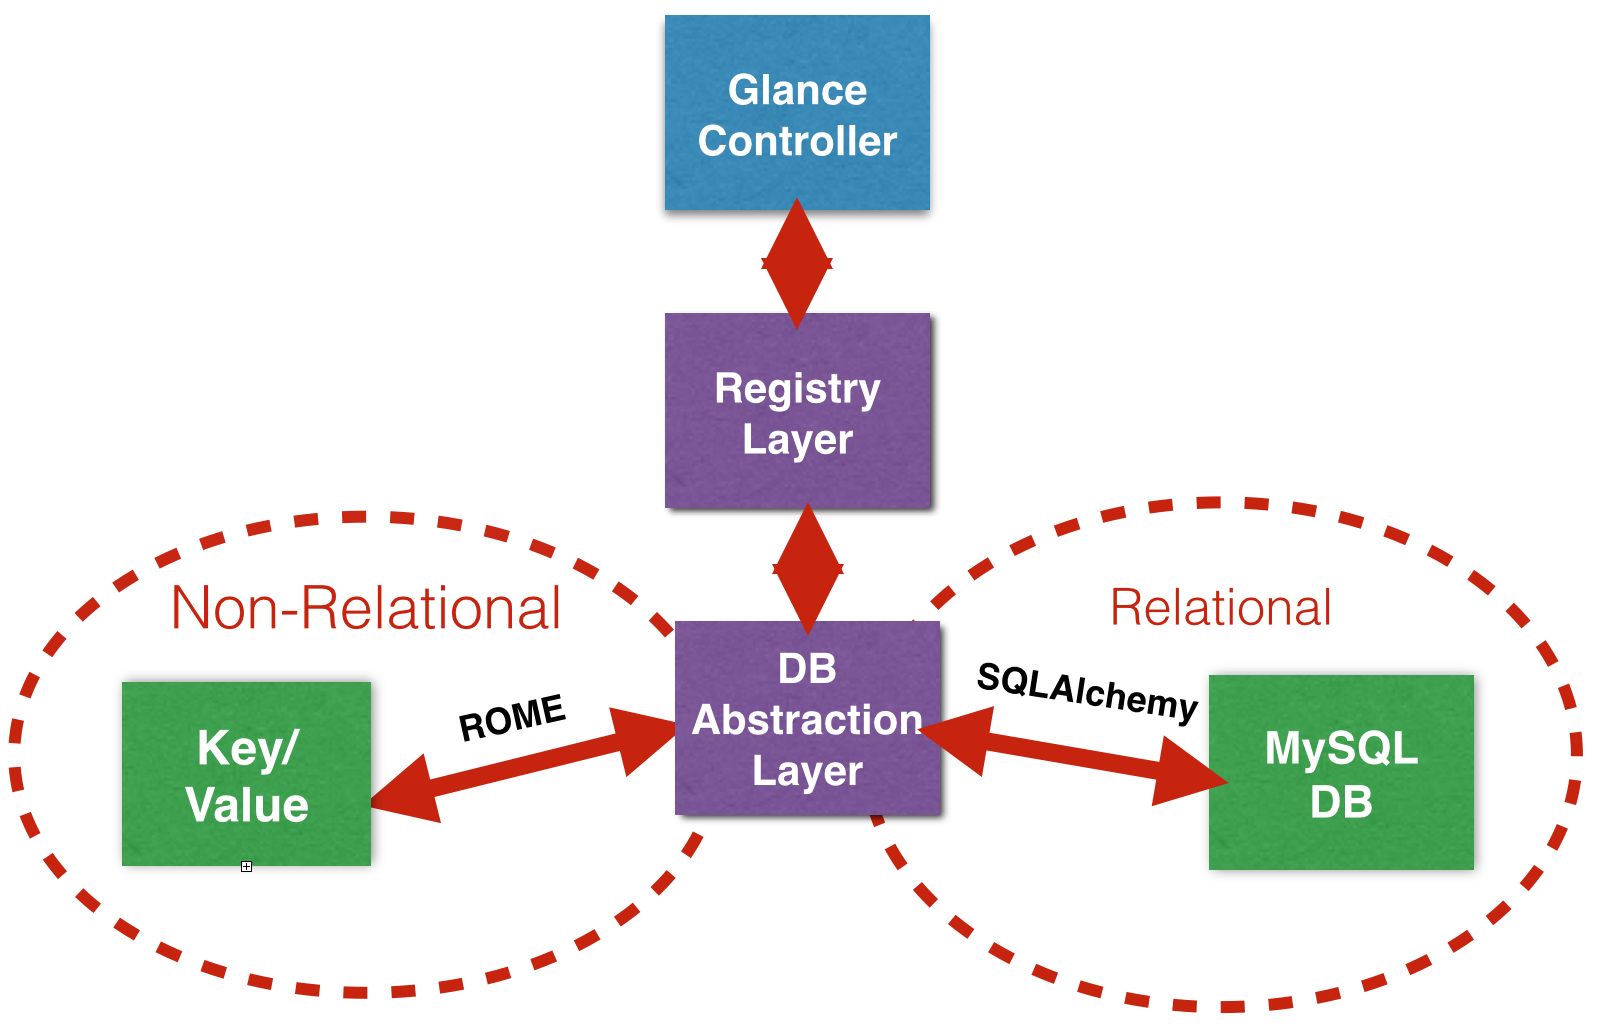
\includegraphics[width=8.5cm]{figures/rome_glance.png}
%\vspace*{-0.8cm}
        \caption{Glance - Software Architecture and DB dependencies.}
        \label{fig:glance_dbs}
%\vspace*{-.3cm}
\end{figure}



%%%
\section{OpenStack for Operating Massively Distributed Clouds\label{sec:perspective_work}}

While advantages and opportunities of massively distributed clouds have been emphasized several years ago~\cite{church:2008, greenberg:2008},
delivering an OpenStack that can natively be extended to distinct sites will create new opportunities.
%Beyond the technical issues we should resolve to finalize our LUC OS, there are
%few challenges that our community should tackle to be able to fully use the
%technical capabilities offered by LUC infrastructures
We present in this section the most important ones and also raise associated challenges (beyond the technical issues we should resolve to finalize our
LUC OS) that our community should tackle to be able to fully use the technical capabilities offered by LUC infrastructures.

%% Beyond the technical issues we should resolve to finalize our LUC OS, a first important
%% challenge our community should shortly address to favor the adoption of such dynamic cloud
%% infrastructures is related to the automatic installation/upgrade of the LUC OS (\ie our
%% revised OpenStack software) throughout the different locations. In such a context,
%% scalability and geo-distribution make the installation/upgrade process more difficult as
%% it would probably require to relocate computations/data between locations in order to be
%% able to update physical servers without impacting the execution of hosted
%% applications. Another issue to investigate is whether it makes sense to extend a
%% deployment between several network operators and how such extensions can be handled. We
%% underline that even for such an extension (the term federation is probably more
%% appropriated in this situation), the two OpenStack systems will join each other to form a
%% single system. Of course security issues should also be addressed that are beyond the
%% scope of this paper. 

From the infrastructure point of view, a positive side-effect of our revised version of OpenStack is that it will natively allow the extension of a
private cloud deployment with remote physical resources. Such a scenario is a strong advantage in comparison to the current hybrid offers as it does
not break the notion of a single deployment operated by the same tenant. Each time a company will face a peak of activity, it will be possible to
provision dedicated servers and attach them to the initial deployment. Those servers can either be provided by dedicated hosting services that have
DCs close to the institution or by directly deploying transportable and containerized server rooms close to the private resources. This notion of
\emph{WANwide elasticity} can be generalized as it will be possible to deploy such containerized server rooms whenever and wherever they will be
mandatory. As examples, we can envision to temporarily deploy IT resources for sport events such as olympic games or for public safety purposes in
case of disasters. Network/Telecom operators will also be able to deploy IT resources on their radio base stations they operate in order to deliver
Fog/Edge computing solutions. The common thread in these use-cases is the possibility of extending an infrastructure wherever needed with additional
resources, the only constraint being to be able to plug the different locations with a backbone that offers enough bandwidth and quality of service to
satisfy network requirements. The major advantage is that such an extension is completely transparent for the administrators/users of the IaaS
solution because they continue to supervise/use the infrastructure as they are used to. The associated challenge our community should shortly address
to deliver such a \emph{Wanwide elasticity} is related to the automatic installation/upgrade of the LUC OS (\ie our revised OpenStack software)
throughout different locations. In such a context, scalability and geo-distribution make the installation/upgrade process more difficult as it
would probably require to relocate computations/data between locations in order to be able to update physical servers without impacting the execution
of hosted applications. Another issue to investigate is whether it makes sense to extend a deployment between several network operators and how such
extensions can be handled. We underline that even for such an extension (the term federation is probably more appropriated in this situation), the two
OpenStack systems will join each other to form a single system. Of course security issues should also be addressed, but they are beyond the scope of this
paper.

From the software point of view, developers will be able to design new applications but also revise major cloud services in order to deliver more
locality aware management of data, computation, and network resources. For instance, it will be possible to deploy on-demand Content Delivery Network
solutions according to specific requirements. Cloud storage services could be revised to mitigate the overheads of transferring data from sources to
the different locations where there are needed. New strategies can favor for instance a pulling mode instead of a pushing one. Nowadays data is
mostly uploaded to the remote clouds without considering whether such data movements are effectively solicited or not. We expect that LUC
infrastructures will enable data to stay as close as possible to the source that generates them and be transferred on the other side only when it will
be solicited. Such strategies will mitigate the cost of transferring data in all social networks for instance. Similarly, developers will be able to
deliver Hadoop-like strategies where computations are launched close to data sources. Such mechanisms will be shortly mandatory to handle the huge
amount of data that Internet of Things will generate. However, delivering the LUC OS will not be sufficient to allow developers to implement such new
services. Our community should start as soon as possible to revise and extend current interfaces (\aka Application Programming Interfaces). In
particular, the new abstractions should allow applications to deal with geo-distribution opportunities and contextual information by using them to
specify deployment/reconfigurations constraints or to develop advanced adaptation scenarios in order to satisfy for instance SLAs.

Finally, the last opportunity we envision is related to the use of renewable energies to partially power each PoP of a LUC infrastructure. Similarly
to follow-the-moon/follow-the sun approach, the use of several sites spread across a large territory will offer opportunities to optimize the use of
distinct energy sources (solar panels, wind turbines). While such an opportunity has been already underlined~\cite{Berral:2014:BGC:2672596.2672694},
the main advantage is once again related to the native capability of our revised OpenStack to federate distinct sites, allowing users to use such a
widely distributed infrastructure in a transparent way while enabling administrators to balance resources in order to benefit from green energy
sources when available (since the system is supervised by a single system we expect that the development of advanced load-balancing strategies
throughout the different servers composing the infrastructure would be simplified).

%%  + Quels sont les challenges/opportunités d'un cloud massivement distribué (SWOT)
%%    - Strengths
%%      + locality aware management of data, computation and network resources
%%      + fault-tolerance (leveraging geo-distributed locations)
%% + Scalability (additional resources can be added to the infrastructure whereever it is, the only constraint is to be able to plug those resources to the LUC infrastructure
%%    - Weaknesses: 
%%  - resource management complexity from the administrator viewpoint (no single view of the whole platform, maintenance of the hardware) 
%%  => Contre balancer avec l'aspect fiabilité dans les forces
%%       - Mutualization of resources is questionable and should be better investigated (economical/energy, on-going work) 
%%       - security (in terms of Human presence) of micro DCs.
%%       - network peering agreement (how can we extend a LUC infrastructure beyond one operator). 
%%    - Opportunites: 
%%      + Revise major cloud services to take benefit from the massively distributed clouds
%%        - Cloud storage locality aware services
%%        - CDN on demand (with particular topology) 
%%     + Create new (and smarter) services (that needs computations capabilities closer to end-users) such as 
%%       - public safety, deploy IT on demand and where it is mandatory and plug it to the whole infrastructure. 
%%       - IOT  
%%          + big computations can be performed as close as possible to the sensors)
%%          + Use of sensors to create new services (smart cities)
%%          +  Mobile computation and data management, cloudlet (i.e. virtual representation of the physical devices follows the localtion of the device, the cloudlet can benefit from the power of the LUC infrastructure while following the device)  
%%          + Advanced data processing enabling the mitigation of data transfer (avoiding the movement of large and useless data items)
%%         + Digital heater farm (Qarnot Computing / Aoterra) - http://www.qarnot-computing.com/technology  / https://www.cloudandheat.com/en/index.html
%%     + Use of renewable energy (follow the moon, follow the sun, follow the wind, ...) 
%%   - Threats: 
%%      + Accouting, billing and monitoring 
%%      + Ensure QoS
%%      + Mise à jour de l'infrastructure (modificiation des couches logicielles à chaud
%%     + Security of communications at every level of the stack. 

 


Cloud Computing has entered our everyday life at a very high speed and huge scale. From classic high performance computing simulations to the management of huge amounts of data coming from mobile devices and sensors, its impact can no longer be minimized. While a lot of progress has already been made in Cloud technologies, there are several concerns that limit the complete adoption of the Cloud Computing paradigm.

In a previous report~\cite{lebre:hal-00854204}, we outlined that, in addition to these concerns, the current model of UC is limited by intrinsic issues. Instead of following the current trend by trying to cope with existing platforms and network interfaces, we proposed to take a different direction by promoting the design of a system that will be efficient and sustainable at the same time, putting knowledge and intelligence directly into the network backbone itself. The innovative approach we introduced will definitely tackle and go beyond Cloud Computing limitations. Our objective is to pave the way for a new generation of Utility Computing that better matches the Internet structure by means of advanced operating mechanisms. By offering the possibility to tightly couple UC servers and network backbones throughout distinct sites and operate them remotely, the LUC OS technology may lead to major changes in the design of UC infrastructures as well as in their environmental impact. The internal mechanisms of the LUC OS should be topology dependent and resources efficient. The natural distribution of the nodes through the different points of presence should be an advantage, which allows to process a request according to its scale: Local requests should be computed locally, while large computations should benefit from a large number of nodes.

The first step toward this highly distributed Cloud infrastructure taking into account locality and network distance is the scheduling of VMs taking into account locality. Thus is this paper, we presented our first building block of our distributed Cloud infrastructure that consists in using P2P algorithms and a vivaldi overlay connected to DVMS, an efficient and flexible VMs scheduler. Our first experiments over Grid'5000 show that, connecting 4 differents sites and scheduling VMs over them, we can gain up to 66\% of inter-sites operations. 

Our future work will consist in ... 

%
% Section: Acknowledgment
%
\section*{Acknowledgments}

Since July 2015, the Discovery initiative is mainly supported through the Inria Project Labs program and the I/O labs, a joint lab between Inria and Orange Labs.
Further information at \href{http://www.inria.fr/en/research/research-fields/inria-project-labs}{http://www.inria.fr/en/research/research-fields/inria-project-labs}
%
% Bibliography
%



\bibliographystyle{abbrv}
\bibliography{main}
\end{document}
